% (find-LATEX "2020-2-C2-subst-trig.tex")
% (defun c () (interactive) (find-LATEXsh "lualatex -record 2020-2-C2-subst-trig.tex" :end))
% (defun C () (interactive) (find-LATEXsh "lualatex 2020-2-C2-subst-trig.tex" "Success!!!"))
% (defun D () (interactive) (find-pdf-page      "~/LATEX/2020-2-C2-subst-trig.pdf"))
% (defun d () (interactive) (find-pdftools-page "~/LATEX/2020-2-C2-subst-trig.pdf"))
% (defun e () (interactive) (find-LATEX "2020-2-C2-subst-trig.tex"))
% (defun o () (interactive) (find-LATEX "2020-2-C2-subst-trig.tex"))
% (defun u () (interactive) (find-latex-upload-links "2020-2-C2-subst-trig"))
% (defun v () (interactive) (find-2a '(e) '(d)))
% (defun d0 () (interactive) (find-ebuffer "2020-2-C2-subst-trig.pdf"))
% (defun cv () (interactive) (C) (ee-kill-this-buffer) (v) (g))
%          (code-eec-LATEX "2020-2-C2-subst-trig")
% (find-pdf-page   "~/LATEX/2020-2-C2-subst-trig.pdf")
% (find-sh0 "cp -v  ~/LATEX/2020-2-C2-subst-trig.pdf /tmp/")
% (find-sh0 "cp -v  ~/LATEX/2020-2-C2-subst-trig.pdf /tmp/pen/")
%     (find-xournalpp "/tmp/2020-2-C2-subst-trig.pdf")
%   file:///home/edrx/LATEX/2020-2-C2-subst-trig.pdf
%               file:///tmp/2020-2-C2-subst-trig.pdf
%           file:///tmp/pen/2020-2-C2-subst-trig.pdf
% http://angg.twu.net/LATEX/2020-2-C2-subst-trig.pdf
% (find-LATEX "2019.mk")
% (find-CN-aula-links "2020-2-C2-subst-trig" "2" "c2m202st" "c2st")
%
% Video:
% (find-ssr-links "c2m202st" "2020-2-C2-subst-trig")
% (code-video     "c2m202stvideo" "$S/http/angg.twu.net/eev-videos/2020-2-C2-subst-trig.mp4")
% (find-c2m202stvideo "0:00")

% «.defs»		(to "defs")
% «.title»		(to "title")
% «.exercicio-1»	(to "exercicio-1")
% «.exercicio-3»	(to "exercicio-3")
% «.exercicio-4»	(to "exercicio-4")
% «.exercicio-5»	(to "exercicio-5")
% «.tabelas»		(to "tabelas")
% «.derivada-f-inv»	(to "derivada-f-inv")
% «.derivada-f-inv-2»	(to "derivada-f-inv-2")
% «.exercicio-6»	(to "exercicio-6")
%
% «.djvuize»	(to "djvuize")

\documentclass[oneside,12pt]{article}
\usepackage[colorlinks,citecolor=DarkRed,urlcolor=DarkRed]{hyperref} % (find-es "tex" "hyperref")
\usepackage{amsmath}
\usepackage{amsfonts}
\usepackage{amssymb}
\usepackage{pict2e}
\usepackage[x11names,svgnames]{xcolor} % (find-es "tex" "xcolor")
\usepackage{colorweb}                  % (find-es "tex" "colorweb")
%\usepackage{tikz}
%
% (find-dn6 "preamble6.lua" "preamble0")
%\usepackage{proof}   % For derivation trees ("%:" lines)
%\input diagxy        % For 2D diagrams ("%D" lines)
%\xyoption{curve}     % For the ".curve=" feature in 2D diagrams
%
\usepackage{edrx15}               % (find-LATEX "edrx15.sty")
\input edrxaccents.tex            % (find-LATEX "edrxaccents.tex")
\input edrxchars.tex              % (find-LATEX "edrxchars.tex")
\input edrxheadfoot.tex           % (find-LATEX "edrxheadfoot.tex")
\input edrxgac2.tex               % (find-LATEX "edrxgac2.tex")
%
%\usepackage[backend=biber,
%   style=alphabetic]{biblatex}            % (find-es "tex" "biber")
%\addbibresource{catsem-slides.bib}        % (find-LATEX "catsem-slides.bib")
%
% (find-es "tex" "geometry")
\usepackage[a6paper, landscape,
            top=1.5cm, bottom=.25cm, left=1cm, right=1cm, includefoot
           ]{geometry}
%
\begin{document}

%\catcode`\^^J=10
%\directlua{dofile "dednat6load.lua"}  % (find-LATEX "dednat6load.lua")

% %L dofile "edrxtikz.lua"  -- (find-LATEX "edrxtikz.lua")
% %L dofile "edrxpict.lua"  -- (find-LATEX "edrxpict.lua")
% \pu

% «defs»  (to ".defs")
% (find-LATEX "edrx15.sty" "colors-2019")
\long\def\ColorRed   #1{{\color{Red1}#1}}
\long\def\ColorViolet#1{{\color{MagentaVioletLight}#1}}
\long\def\ColorViolet#1{{\color{Violet!50!black}#1}}
\long\def\ColorGreen #1{{\color{SpringDarkHard}#1}}
\long\def\ColorGreen #1{{\color{SpringGreenDark}#1}}
\long\def\ColorGreen #1{{\color{SpringGreen4}#1}}
\long\def\ColorGray  #1{{\color{GrayLight}#1}}
\long\def\ColorGray  #1{{\color{black!30!white}#1}}
\long\def\ColorBrown #1{{\color{Brown}#1}}
\long\def\ColorBrown #1{{\color{brown}#1}}
\long\def\ColorOrange#1{{\color{orange}#1}}

\long\def\ColorShort #1{{\color{SpringGreen4}#1}}
\long\def\ColorLong  #1{{\color{Red1}#1}}

\def\frown{\ensuremath{{=}{(}}}
\def\True {\mathbf{V}}
\def\False{\mathbf{F}}
\def\D    {\displaystyle}

\def\drafturl{http://angg.twu.net/LATEX/2020-2-C2.pdf}
\def\drafturl{http://angg.twu.net/2020.2-C2.html}
\def\draftfooter{\tiny \href{\drafturl}{\jobname{}} \ColorBrown{\shorttoday{} \hours}}

\def\St{\sen θ}
\def\Ct{\cos θ}
\def\Sqs{\sqrt{1-s^2}}

\def\pfo #1{\ensuremath{\mathsf{[#1]}}}
\def\pfot#1{\ensuremath{\textsf{[#1]}}}
\def\veq{\rotatebox{90}{$=$}}
\def\Rd{\ColorRed}


%  _____ _ _   _                               
% |_   _(_) |_| | ___   _ __   __ _  __ _  ___ 
%   | | | | __| |/ _ \ | '_ \ / _` |/ _` |/ _ \
%   | | | | |_| |  __/ | |_) | (_| | (_| |  __/
%   |_| |_|\__|_|\___| | .__/ \__,_|\__, |\___|
%                      |_|          |___/      
%
% «title»  (to ".title")
% (c2m202stp 1 "title")
% (c2m202st    "title")

\thispagestyle{empty}

\begin{center}

\vspace*{1.2cm}

{\bf \Large Cálculo 2 - 2020.2}

\bsk

Aula nn: substituição trigonométrica

\bsk

Eduardo Ochs - RCN/PURO/UFF

\url{http://angg.twu.net/2020.2-C2.html}

\end{center}

\newpage

%\printbibliography



No final destes slides aqui

\ssk

{\footnotesize

% (c2m202isp 20 "subst-trig-exemplo")
% (c2m202is     "subst-trig-exemplo")
% http://angg.twu.net/LATEX/2020-2-C2-int-subst.pdf#page=19
\url{http://angg.twu.net/LATEX/2020-2-C2-int-subst.pdf\#page=19}

}

nós começamos a ver como fazer certas

``substituições trigonométricas''...

E nós vimos que:
%
$$\D \ints {s \Sqs} = \intth {(\Ct)^2 \St}$$

\newpage

% «exercicio-1»  (to ".exercicio-1")
% (c2m202stp 3 "exercicio-1")
% (c2m202st    "exercicio-1")

{\bf Exercício 1.}

Generalize a igualdade dos slides passados.

Mais precisamente: digamos que $s=\senθ$, $α,β∈\Z$.

Encontre fórmulas para $γ$ e $δ$ em
%
$$\D \ints {s^α (\Sqs)^β} = \intth {(\Ct)^γ (\St)^δ}$$

que façam esta igualdade ser verdadeira $(∀α,β∈\Z)$.

\bsk

{\bf Exercício 2.}

Faça o mesmo para:

$$\D \intt {t^α (\sqrt{1+t^2})^β} = \intth {(\Ct)^γ (\St)^δ}$$

Aqui a substituição é $t=\tanθ$

(e os detalhes são mais difíceis)...


\newpage

% «exercicio-3»  (to ".exercicio-3")

{\bf Exercício 3.}

Usando o que você aprendeu no exercício 1,

ajuste $α$ e $β$ aqui para que isto seja verdade:

$$\D \ints {s^α (\Sqs)^β} = \intth {(\Ct)^0 (\St)^0}$$

\newpage

% «exercicio-4»  (to ".exercicio-4")
% (c2m202stp 5 "exercicio-4")
% (c2m202st    "exercicio-4")

{\bf Exercício 4.}

Expanda esta série de igualdades aqui ---

usando os valores adequados para $α$ e $β$, óbvio ---

pra obter uma série de igualdades que seja convincente pra

alguém que tem pouca prática com integração por substituição:
%
$$\begin{array}{rclr}
  \D \ints {s^α (\Sqs)^β} &=& \D \intth {(\Ct)^0 (\St)^0} & \quad(s=\senθ)\\
                          &=& \D \intth 1 \\[12pt]
                          &=& θ \\
                          &=& \arcsen s \\
  \end{array}
$$

\newpage

% «exercicio-5»  (to ".exercicio-5")
% (c2m202stp 6 "exercicio-5")
% (c2m202st    "exercicio-5")

{\bf Exercício 5.}

A maioria dos livros de Cálculo têm uma ``tabela de derivadas'' e uma
``tabela de integrais''... as do próximo slide são do APEX Calculus.
Um jeito de \ColorRed{usar} as fórmulas dessas tabelas é dar nomes pra
elas e usar o `$[:=]$'. Por exemplo:

$$\begin{array}{rclr}
  \pfo{ApexDiff12}
    &=& \D \left( \frac{d}{dx} \log_a x = \frac{1}{\ln a} · \frac 1x \right) \\[12pt]
  \pfo{ApexDiff12}[a:=99]
    &=& \D \left( \frac{d}{dx} \log_{99} x = \frac{1}{\ln 99} · \frac 1x \right) \\
  \end{array}
$$

\msk

Encontre uma fórmula da tabela de derivadas do APEX Calculus e uma da
tabela de integrais dele que se parecem com o que você descobriu no
exercício 4.

\msk

Nós vamos aprender como \ColorRed{demonstrar} muitas fórmulas dessas
tabelas.

\newpage

% «tabelas»  (to ".tabelas")
% (c2m202stp 7 "tabelas")
% (c2m202st    "tabelas")

\vspace*{-1.5cm}

% (find-latexscan-links "C2" "apex_calculus_table_of_integrals")
% (find-xpdf-page "~/LATEX/2020-2-C2/apex_calculus_table_of_integrals.pdf")
%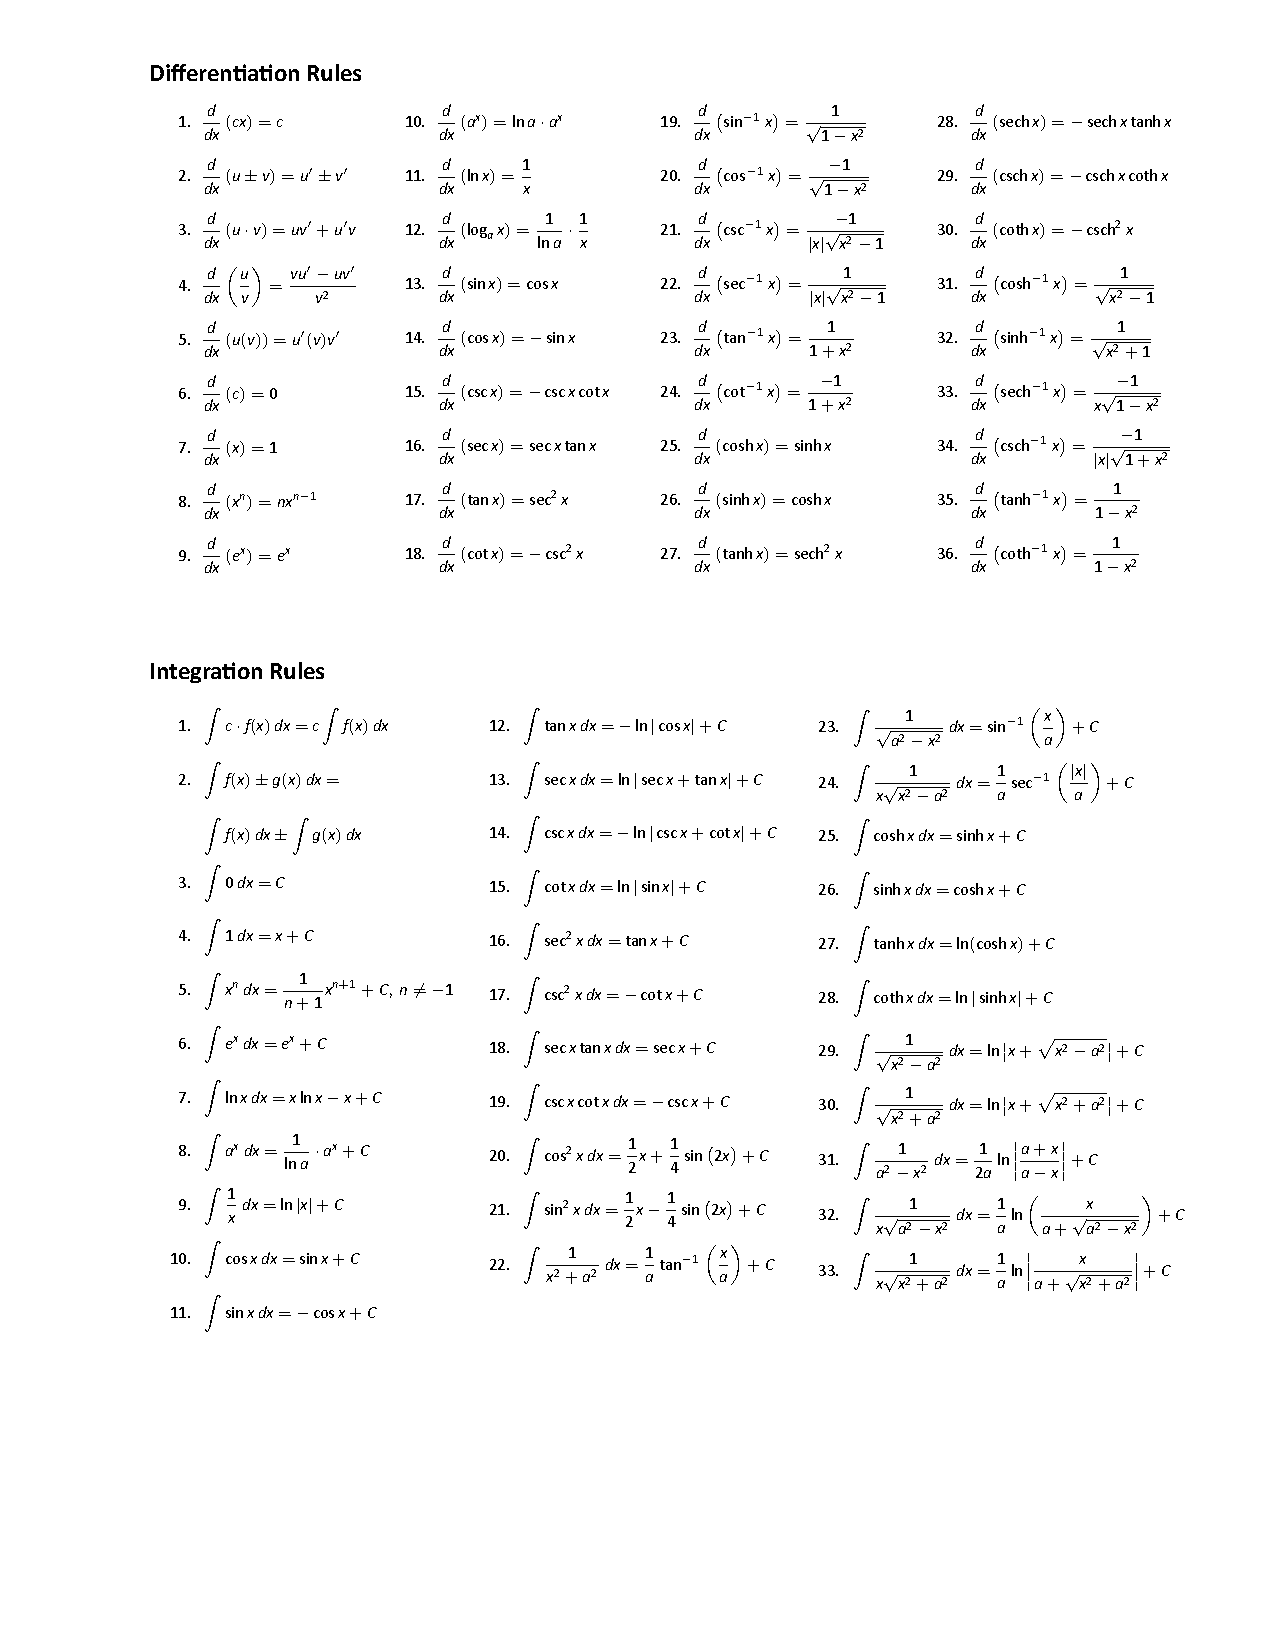
\includegraphics[height=8cm]{2020-2-C2/apex_calculus_table_of_integrals.pdf}
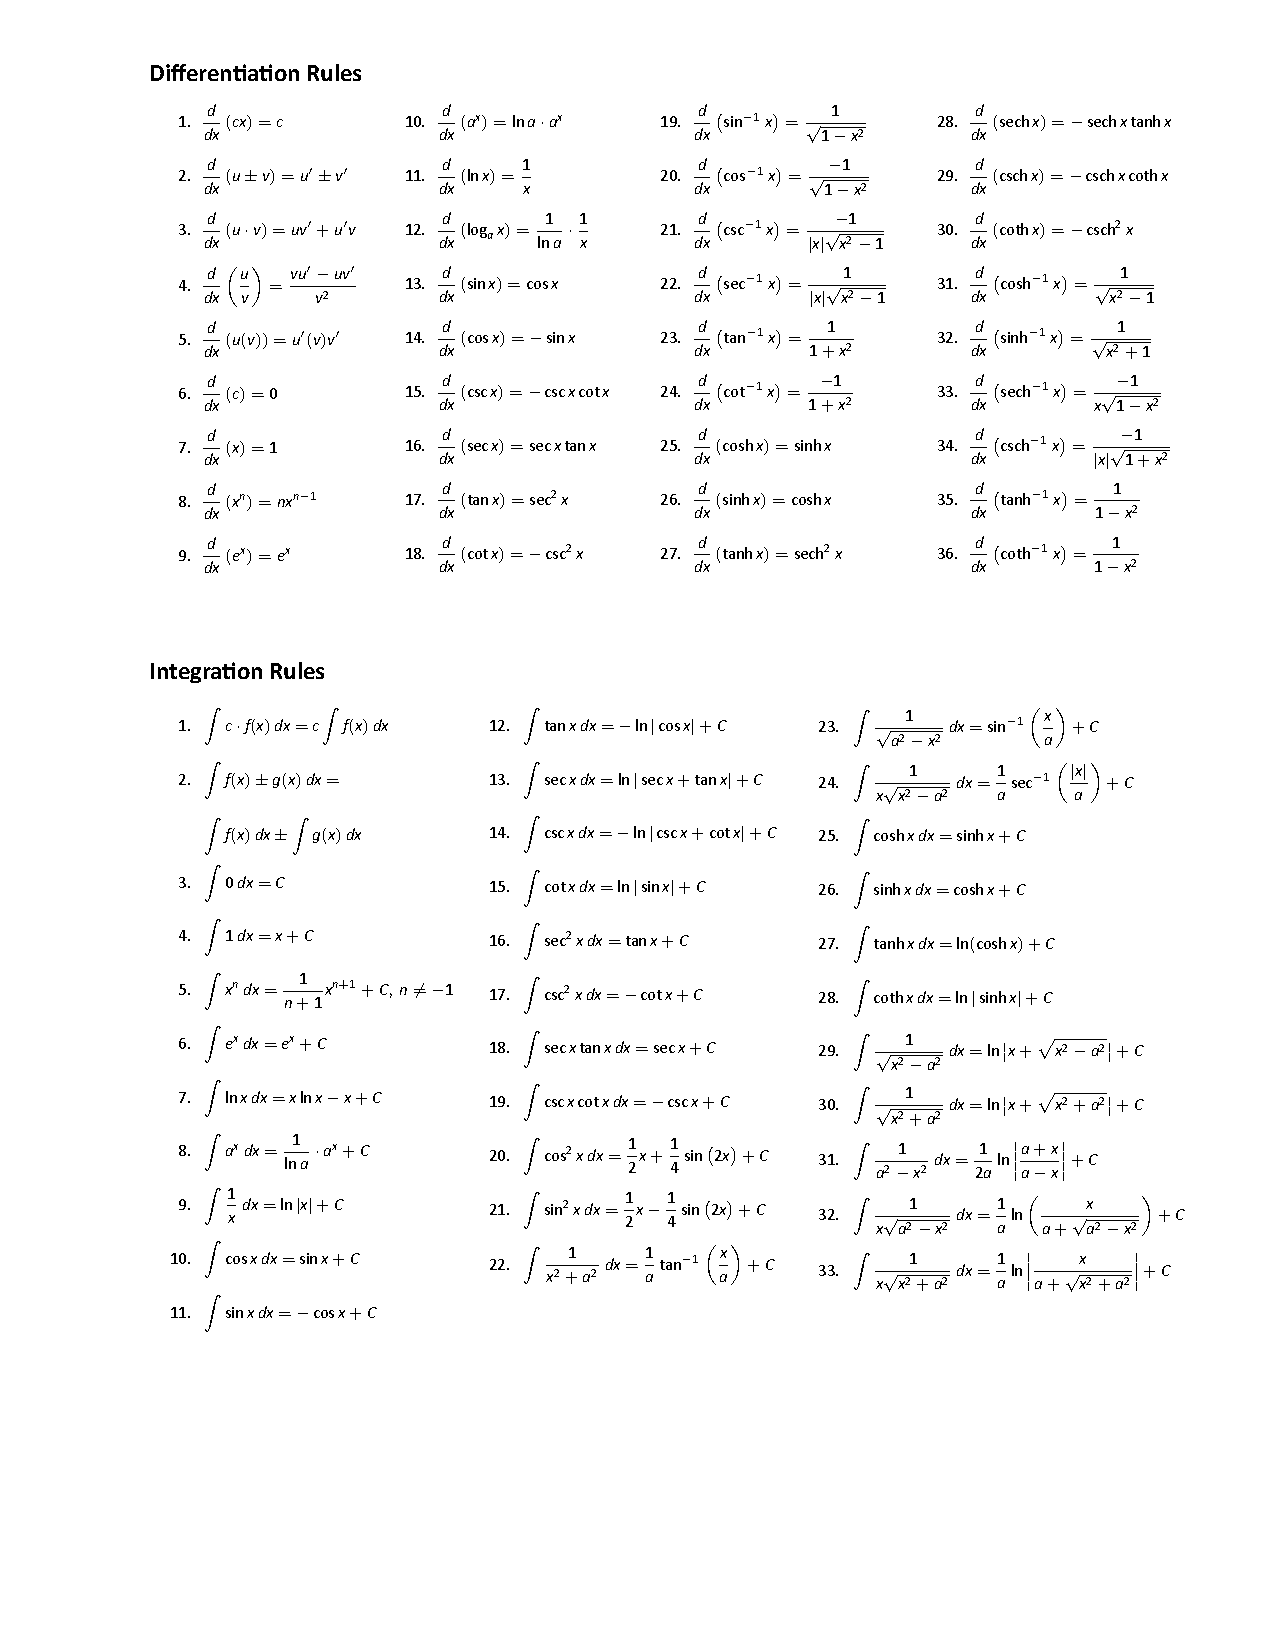
\includegraphics[width=9cm]{2020-2-C2/apex_calculus_table_of_integrals.pdf}


\newpage

% «derivada-f-inv»  (to ".derivada-f-inv")
% (c2m202stp 8 "derivada-f-inv")
% (c2m202st    "derivada-f-inv")

{\bf Derivada da função inversa}

Antes de continuar vamos rever uma fórmula que vocês devem ter visto
bem superficialmente em Cálculo 1: a fórmula para a derivada da função
inversa. A \ColorRed{demonstração} dela é esta aqui:

\def\DFID{
  \left(
  \begin{array}{l}
  \text{Se $f(g(x))=x$ então:} \\[10pt]
  %
  \frac{d}{dx} f(g(x)) = \frac{d}{dx} x = 1 \\
  \phantom{mm}\veq \\
  f'(g(x))g'(x) \\[10pt]
  %
  \text{Portanto:} \\
  g'(x) = \D \frac{1}{f'(g(x))} \\
  \end{array}
  \right)
  }

$$\pfo{DIFD} = \DFID
$$


\newpage

% «derivada-f-inv-2»  (to ".derivada-f-inv-2")
% (c2m202stp 8 "derivada-f-inv")
% (c2m202st    "derivada-f-inv")

{\bf Derivada da função inversa (2)}

Um exemplo:

\msk

$\scalebox{0.9}{$
  \DFID
  \bmat{ f(u):=e^u \\ f'(u):=e^u \\ g(x):=\ln x \\ g'(x):=\ln' x } =
  \left(
  \begin{array}{l}
  \text{Se $e^{\ln x}=x$ então:} \\[10pt]
  %
  \frac{d}{dx} e^{\ln x} = \frac{d}{dx} x = 1 \\
  \phantom{mm}\veq \\
  e^{\ln x} \ln' x \\[10pt]
  %
  \text{Portanto:} \\
  \ln' x = \D \frac{1}{e^{\ln x}} \\
  \end{array}
  \right)
  $}
$

\bsk

Neste caso a \ColorRed{hipótese} do teorema da DFI é verdadeira,

então $\ln' x = \frac{1}{e^{\ln x}}$, e portanto $\ln' x = \frac 1x$.

\newpage

% «exercicio-6»  (to ".exercicio-6")
% (c2m202stp 10 "exercicio-6")
% (c2m202st     "exercicio-6")

{\bf Exercício 6.}

Calcule o resultado desta substituição:

$\pfo{DFID} \bmat{f(u) := \sen u \\ f'(u) := \cos u \\ g(x) := \arcsen s \\ g'(x) := \arcsen' s}$

\bsk

{\bf Exercício 7.}

Dê um nome para a \ColorRed{igualdade} que você acabou de obter.

Lembre que você \ColorRed{pode} usar nomes péssimos e/ou nada a ver,

como \pfot{Drácula}, \pfot{agshTg7s}, \pfot{Aliás}, \pfot{Não}, etc.

\bsk

{\bf Exercício 8.}

Dá pra usar identidades trigonométricas pra transformar o que você

obteve nos exercícios 6 e 7 numa demonstração do \pfo{ApexDiff19}.

Tente descobrir como.



\GenericWarning{Success:}{Success!!!}  % Used by `M-x cv'

\end{document}

%  ____  _             _         
% |  _ \(_)_   ___   _(_)_______ 
% | | | | \ \ / / | | | |_  / _ \
% | |_| | |\ V /| |_| | |/ /  __/
% |____// | \_/  \__,_|_/___\___|
%     |__/                       
%
% «djvuize»  (to ".djvuize")
% (find-LATEXgrep "grep --color -nH --null -e djvuize 2020-1*.tex")

 (eepitch-shell)
 (eepitch-kill)
 (eepitch-shell)
# (find-fline "~/2020.2-C2/")
# (find-fline "~/LATEX/2020-2-C2/")
# (find-fline "~/bin/djvuize")

cd /tmp/
for i in *.jpg; do echo f $(basename $i .jpg); done

f () { rm -fv $1.png $1.pdf; djvuize $1.pdf }
f () { rm -fv $1.png $1.pdf; djvuize WHITEBOARDOPTS="-m 1.0" $1.pdf; xpdf $1.pdf }
f () { rm -fv $1.png $1.pdf; djvuize WHITEBOARDOPTS="-m 0.5" $1.pdf; xpdf $1.pdf }
f () { rm -fv $1.png $1.pdf; djvuize WHITEBOARDOPTS="-m 0.25" $1.pdf; xpdf $1.pdf }
f () { cp -fv $1.png $1.pdf       ~/2020.2-C2/
       cp -fv        $1.pdf ~/LATEX/2020-2-C2/
       cat <<%%%
% (find-latexscan-links "C2" "$1")
%%%
}

f 20201213_area_em_funcao_de_theta
f 20201213_area_em_funcao_de_x
f 20201213_area_fatias_pizza

f apex_calculus_table_of_integrals


%  __  __       _        
% |  \/  | __ _| | _____ 
% | |\/| |/ _` | |/ / _ \
% | |  | | (_| |   <  __/
% |_|  |_|\__,_|_|\_\___|
%                        
% <make>

 (eepitch-shell)
 (eepitch-kill)
 (eepitch-shell)
# (find-LATEXfile "2019planar-has-1.mk")
make -f 2019.mk STEM=2020-2-C2-subst-trig veryclean
make -f 2019.mk STEM=2020-2-C2-subst-trig pdf

% Local Variables:
% coding: utf-8-unix
% ee-tla: "c2m202st"
% End:
